\documentclass[]{article}
\usepackage{lmodern}
\usepackage{graphicx}
\usepackage{caption}
\usepackage{subcaption}
\usepackage{adjustbox}
\usepackage{amssymb,amsmath}
\usepackage{ifxetex,ifluatex}
\usepackage{listings}
\usepackage[T1]{fontenc}
\usepackage[utf8]{inputenc}
\usepackage{microtype}
\usepackage[margin=1in]{geometry}
\usepackage{hyperref}
\usepackage{framed}
\usepackage{grffile}
\makeatletter
\def\maxwidth{\ifdim\Gin@nat@width>\linewidth\linewidth\else\Gin@nat@width\fi}
\def\maxheight{\ifdim\Gin@nat@height>\textheight\textheight\else\Gin@nat@height\fi}
\makeatother
% Scale images if necessary, so that they will not overflow the page
% margins by default, and it is still possible to overwrite the defaults
% using explicit options in \includegraphics[width, height, ...]{}
\setkeys{Gin}{width=\maxwidth,height=\maxheight,keepaspectratio}
\setlength{\parindent}{0pt}
\setlength{\parskip}{6pt plus 2pt minus 1pt}
\setlength{\emergencystretch}{3em}  % prevent overfull lines
\providecommand{\tightlist}{%
  \setlength{\itemsep}{0pt}\setlength{\parskip}{0pt}}

%%% Change title format to be more compact
\usepackage{titling}

% Create subtitle command for use in maketitle
\newcommand{\subtitle}[1]{
  \posttitle{
    \begin{center}\large#1\end{center}
    }
}

\setlength{\droptitle}{-2em}
  \title{MSAN 601 - Homework 3}
  \pretitle{\vspace{\droptitle}\centering\huge}
  \posttitle{\par}
  \author{Andre Guimaraes Duarte}
  \preauthor{\centering\large\emph}
  \postauthor{\par}
  \predate{\centering\large\emph}
  \postdate{\par}
  \date{September 19, 2016}
  
% Redefines (sub)paragraphs to behave more like paragraphs
\ifx\paragraph\undefined\else
\let\oldparagraph\paragraph
\renewcommand{\paragraph}[1]{\oldparagraph{#1}\mbox{}}
\fi
\ifx\subparagraph\undefined\else
\let\oldsubparagraph\subparagraph
\renewcommand{\subparagraph}[1]{\oldsubparagraph{#1}\mbox{}}
\fi

\usepackage{color}
\usepackage{siunitx}

%%%%%%%%%%%%%%%%%%%%%%%%%%%%%%%%%%%%%%%%%%%%%%%%%%%%%%%%%%%%%%%%%%%%%%%%%%%%%%%%%%%%%%%%%%%%%%%%%%%%%%%%%%%%%%%%%%%%%%%
\begin{document}
\maketitle

\paragraph{\Large Question 1}\normalsize

For a multiple regression mode, $R^2$ does not have any unit.

In fact, we have $R^2 = \frac{SSR}{SSTO} = \frac{b'X'Y - (\frac{1}{n})Y'JY}{Y'Y - (\frac{1}{n})Y'JY}$. The numerator and denominator of this fraction have the same units: the units of $Y$ squared. Therefore, they cancel out in the division, and $R^2$ has no units.

\paragraph{\Large Question 2}\normalsize

Let's call $Y = \beta_0 + \beta_1 X_1 + \beta_2 X_2 + \beta_3 X_3 + \epsilon$ model 1 and $Y = \beta_0 + \beta_1 X_1 + \beta_2 X_2 + \beta_3 X_3 + \beta_4 X_4 + \epsilon$ model 2, where $X_4$ is an irrelevant variable.

Since model 2 has one more explanatory variable than model 1 ($X_4$), we can say that $R^2_2 \geq R^2_1$. Indeed, $R^2$ is a monotonically increasing function, so adding another explanatory variable to model 1 can only explain more error, not less.

However, since $X_4$ is irrelevant for predicting $Y$, we can safely assume that $R^2_{a,2} < R^2_{a,1}$. Indeed, model 2 has an extra variable ($p_2 > p_1$) that does not make the model better (it is irrelevant). The potential increase in SSR is penalized by the increase in $p$, which leads to a decrease in $R^2_a$.

\paragraph{\Large Question 3}\normalsize

The four SLR models are run and the results are summarized in Table \ref{q3}. The scatterplots are shown in Figure \ref{fig3}.

\begin{table}[!ht]
\caption{Summary of results for SLR on \texttt{anscombe} data.}
\begin{center}
\begin{tabular}{|c|c|c|c|}
\hline
Regression function & $R^2$ & $R^2_a$ & p-valule ($b_1$) \\
\hline
$Y_1 = 3.0001 + 0.5001 X_1$ & 0.6665 & 0.6295 & 0.00217 \\
$Y_2 = 3.0010 + 0.5000 X_2$ & 0.6662 & 0.6292 & 0.00218 \\
$Y_3 = 3.0025 + 0.4997 X_3$ & 0.6663 & 0.6292 & 0.00218 \\
$Y_4 = 3.0017 + 0.4999 X_4$ & 0.6667 & 0.6297 & 0.00216 \\
\hline
\end{tabular}
\end{center}
\label{q3}
\end{table}

\begin{figure}[!ht] 
  \begin{minipage}[b]{0.5\linewidth}
    \centering
    \includegraphics[width=\linewidth]{q3-1.png} 
    %\caption{Initial condition} 
    \vspace{2ex}
  \end{minipage}%%
  \begin{minipage}[b]{0.5\linewidth}
    \centering
    \includegraphics[width=\linewidth]{q3-2.png} 
    %\caption{Rupture} 
    \vspace{2ex}
  \end{minipage} 
  \begin{minipage}[b]{0.5\linewidth}
    \centering
    \includegraphics[width=\linewidth]{q3-3.png} 
    %\caption{DFT, Initial condition} 
    \vspace{2ex}
  \end{minipage}%% 
  \begin{minipage}[b]{0.5\linewidth}
    \centering
    \includegraphics[width=\linewidth]{q3-4.png} 
    %\caption{DFT, rupture} 
    \vspace{2ex}
  \end{minipage}
  \caption{Scatterplots for SLR on \texttt{anscombe} data.}
  \label{fig3} 
\end{figure}

We can see from Table \ref{q3} that all four models are almost identical: the regression functions are equal to the hundredths, the coefficients of determination $R^2$ and $R^2_a$ are identical, and $b_1$ is significant in all cases. However, the scatterplots in Figure \ref{fig3} clearly show that the data is not at all similar between the four sets. This shows that looking at the data before developing a model is very important, as you may reach a "good" result even if the approach was not ideal.

\paragraph{\Large Question 4}\normalsize

For this exercise, we use the file \texttt{extraColumnsOdRandomData.csv} in order to evaluate the influence of additional explanatory variables in the regression model on the coefficient of determination $R^2$ and the adjusted coefficient of determination $R^2_a$.

In file \texttt{HW3.R}, function \texttt{q4} takes in a data frame as a parameter and runs all necessary linear regression models. The coefficients $R^2$ and $R^2_a$ are stored and returned in a data frame, and the scatterplot that shows the value of these coefficients with respect to the number of independent variables is created and saved as \texttt{q4.png}. This scatterplot is shown in Figure \ref{fig4}.

\begin{figure}[!ht]
\centering
\includegraphics[width=\linewidth]{q4.png}
\caption{Scatterplot of $R^2$ and $R^2_a$ with respect to the number of independent variables used in the linear regression model for \texttt{extraColumnsOdRandomData.csv}}
\label{fig4}
\end{figure}

We can see that $R^2$ is monotonically increasing as more independent variables are added to the linear regression model. However, $R^2_a$ reaches a maximum when only the first two variables are included (age and hip width). All other variables are random by construction, and therefore don't explain much additional error, which causes the adjusted coefficient of determination to decrease (the decrease in SSE is not enough to balance out the increase in $p$). 

\paragraph{\Large Question 5}\normalsize
\subparagraph{\Large a}\normalsize

We create the following linear model:

$\text{Bill} = \beta_0 + \beta_1 \text{Temp} + \beta_2 \text{HDD}+ \beta_3 \text{CDD}+ \beta_4 \text{Size} + \beta_5 \text{Meter} + \beta_6 \text{Pump}_1 + \beta_7 \text{Pump}_2 + \epsilon$.

We get the parameter estimations shown in Table \ref{q5a}. In addition, we get $R^2 = 0.5477$ and $R^2_a = 0.5192$. Finally, the model is significant (for $\alpha = 5\%$) since the p-value for the F-test is $< 2.2e-16$.

\begin{table}[!ht]
\caption{Summary of results for \texttt{electricBillData}.}
\begin{center}
\begin{tabular}{|c|c|c|}
\hline
Estimator & Value & p-value \\
\hline
$b_0$ & 275.86620 & 0.14943 \\
$b_1$ & -4.70047 & 0.09799 \\
$b_2$ & -0.07800 & 0.38537 \\
$b_3$ & 0.17989 & 0.11499 \\
$b_4$ & 28.61484 & 0.00966 \\
$b_5$ & 84.25307 & 2.16e-07 \\
$b_6$ & -26.92299 & 0.00883 \\
$b_7$ & -34.18379 & 0.01289 \\
\hline
\end{tabular}
\end{center}
\label{q5a}
\end{table}

\subparagraph{\Large b}\normalsize

The $R^2$ for this model is $0.5477$. This means that $54.77\%$ of the variance in the bill is explained by the explanatory variables.

\subparagraph{\Large c}\normalsize

We can see from the results in Table \ref{q5a} that the p-value for the parameter estimations related to the electric meter and the two heat pumps ($b_5$, $b_6$, and $b_7$ respectively) are significant with $\alpha = 5\%$. We can conlude that they make a statistically significant impact on the electric bill.

By having a new electric meter, we expect the mean value of the bill to increase by $\$84.25$ holding all other explanatory variables constant.

By having a new heat pump 1, we expect the mean value of the bill to decrease by $\$26.92$ holding all other explanatory variables constant.

By having a new heat pump 2, we expect the mean value of the bill to decrease by $\$34.18$ holding all other explanatory variables constant.

\subparagraph{\Large d}\normalsize

From the results in Table \ref{q5a}, we can see that the p-values associated to the parameter estimations for Size and HDD ($b_4$ and $b_2$ respectively) are $0.00966$ and $0.38537$. We can see that the number of heating degree days is not significant (with $\alpha = 5\%$), while the family size is significant. Therefore the number of family members in the house is a more significant factor than the number of heating degree days for explaining the final size of the bill. 

In my opinion, this result does not concern me. Having more people in the house will indubitably raise the size of the electric bill. However, I would also expect the number of heating days to have a significant impact on the final electric bill.

\subparagraph{\Large e}\normalsize

The correlation matrix between Temp, HDD, and CDD is given in Table \ref{q5e}.

\begin{table}[!ht]
\caption{Correlation table between Temp, HDD, CDD.}
\begin{center}
\begin{tabular}{|c|c|c|c|}
\cline{2-4}
\multicolumn{1}{c|}{} & TEMP & HDD & CDD \\
\hline
TEMP & 1.0000000& -0.9845646 & 0.8511846\\
HDD&-0.9845646 & 1.0000000& -0.7581836\\
CDD&0.8511846 &-0.7581836 & 1.0000000\\
\hline
\end{tabular}
\end{center}
\label{q5e}
\end{table}

We can see from Table \ref{q5e} that the average temperature and the number of heating degree days are highly correlated ($r = -0.9845646$). This result suggests that the model should be updated in order to either drop one of the two variables or include their correlation.

\subparagraph{\Large f}\normalsize

We now remove Temp from the previous model and obtain the following model:

$\text{Bill} = \beta_0 + \beta_1 \text{HDD}+ \beta_2 \text{CDD}+ \beta_3 \text{Size} + \beta_4 \text{Meter} + \beta_5 \text{Pump}_1 + \beta_6 \text{Pump}_2 + \epsilon$.

We get the parameter estimations shown in Table \ref{q5f}. In addition, we get $R^2 = 0.5364$ and $R^2_a = 0.5115$. Finally, the model is significant (for $\alpha = 5\%$) since the p-value for the F-test is $< 2.2e-16$.

\begin{table}[!ht]
\caption{Summary of results for \texttt{electricBillData}.}
\begin{center}
\begin{tabular}{|c|c|c|}
\hline
Estimator & Value & p-value \\
\hline
$b_0$ & -32.800483 & 0.45721 \\
$b_1$ & 0.070064 & 3.88e-08 \\
$b_2$ & 0.006927 & 0.88048 \\
$b_3$ & 29.126205 & 0.00896 \\
$b_4$ & 84.092190 & 2.71e-07 \\
$b_5$ & -26.931993 & 0.00933 \\
$b_6$ & -33.709284 & 0.01489 \\
\hline
\end{tabular}
\end{center}
\label{q5f}
\end{table}

We can see that now the number of heating days is a relevant variable in the model (the p-value associated to its parameter estimator, $b_1$, is $3.88e-08$) with $\alpha = 5\%$.

The number of cooling days is not a significant factor in estimating the size of the electric bill for this data (p-value is $0.88048 > 0.05$ for $b_2$). The authors of this data set are from Indiana State University. Their data likely comes from Indiana houses, and the weather there does not usually get too hot for people to have to use the AC, hence the lack of impact on the final electric bill.

\paragraph{\Large Question 6}\normalsize
\subparagraph{\Large 1}\normalsize

We create the model (AFC: Available Facilities and Services):

$Nurses = \beta_0 + \beta_1 \text{AFC} + \beta_2 \text{AFC} + \epsilon$.

We get the parameter estimations shown in Table \ref{q6_1}. In addition, we get $R^2 = 0.6569$ and $R^2_a = 0.6507$. Finally, the model is significant (for $\alpha = 5\%$) since the p-value for the F-test is $< 2.2e-16$.

\begin{table}[!ht]
\caption{Summary of results for \texttt{SENIC\_data}.}
\begin{center}
\begin{tabular}{|c|c|c|}
\hline
Estimator & Value & p-value \\
\hline
$b_0$ & 33.54823 & 0.51544 \\
$b_1$ & -1.66613 & 0.49519 \\
$b_2$ & 0.10116 & 0.00032 \\
\hline
\end{tabular}
\end{center}
\label{q6_1}
\end{table}

We can see from Table \ref{q6_1} that $b_1$ is not significant with $\alpha = 5\%$.

We also plot the residuals against the fitted values using the \texttt{residualPlot} function from the \texttt{car} package. The image is shown in Figure \ref{fig6_1}.

\begin{figure}[!ht]
\centering
\includegraphics[width=.8\linewidth, angle=-90]{q6_1.eps}
\caption{Residual plot for \texttt{SENIC\_data}.}
\label{fig6_1}
\end{figure}

The residual plot in Figure \ref{fig6_1} seems to show heteroskedasticity of the residuals. The variance for the residuals on the right seems bigger than on the left of the plot.

\subparagraph{\Large 2}\normalsize

For the second-order regression model, we get $R^2 = 0.6569$. For the first-order regression model, we obtain $R^2 = 0.6139$. The addition of the quadratic term in the model increases the coefficient of determination by $0.043$ i.e. it explains an additional $4.3\%$ of the variation in the number of nurses. 

\subparagraph{\Large 3}\normalsize

When added, the quadratic term explains an additional $4.3\%$ of the error not explained by the first-power term.

\subparagraph{\Large 4}\normalsize

From Table \ref{q6_1}, we can see that the p-value associated to the estimator of the quadratic term is $0.00032 < 0.01$. Therefore, we reject the null hypothesis $H_0$ that its estimator is null and accept the alternative: $b_2 \neq 0$. We conclude to keep this term in the model. We expect to see an increase of $0.10116$ nurses on average for an increase of one unit of the square of the available facilities and services, holding all other variables constant.

\paragraph{\Large Question 7}\normalsize

The probable cause of this error, based on its name (\texttt{XTRANSPOSE\_X\_SINGULAR}), likely comes from using the formula $\hat{Y} = HY$ to find $\hat{Y}$. Here, $H$ is the hat matrix $H = X(X'X)^{-1}X'$. If $X'X$ is singular, then it is not invertible. Therefore $H$ cannot be computed, leading to the error shown.

\paragraph{\Large Question 8}\normalsize
\subparagraph{\Large 1}\normalsize

We create the following linear model:

$\text{LoS} = \beta_0 + \beta_1 \text{Age} + \beta_2 \text{RCR}+ \beta_3 \text{AVC}+ \beta_4 \text{AFS} + \beta_5 \text{NE} + \beta_6 \text{NC}_1 + \beta_7 \text{S}_2 + \epsilon$,

where LoS: Length of Stay, RCR: Routine Culturing Ratio, AVC: Average Daily Census, AFS: Available Facilities and Services, NE, NC, S: Regions.

We get the parameter estimations shown in Table \ref{q8}. In addition, we get $R^2 = 0.4981$ and $R^2_a = 0.4647$. Finally, the model is significant (for $\alpha = 5\%$) since the p-value for the F-test is $2.283e-13$.

\begin{table}[!ht]
\caption{Summary of results for \texttt{electricBillData}.}
\begin{center}
\begin{tabular}{|c|c|c|}
\hline
Estimator & Value & p-value \\
\hline
$b_0$ & 2.047830 & 0.26124 \\
$b_1$ & 0.103691 & 0.00134 \\
$b_2$ & 0.040302 & 0.00578 \\
$b_3$ & 0.006600 & 7.92e-06 \\
$b_4$ & -0.020761 & 0.15148 \\
$b_5$ & 2.149988 & 9.37e-06 \\
$b_6$ & 1.190333 & 0.00757 \\
$b_7$ & 0.633478 & 0.14143 \\
\hline
\end{tabular}
\end{center}
\label{q8}
\end{table}

\subparagraph{\Large 2}\normalsize

From Table \ref{q8}, we can see that the p-value associated to the parameter estimator for Routine Culturing Ratio ($b_2$) is $0.00578 < 0.05$. Therefore, we reject the null hypothesis $H_0$ that the parameter is null, and accept the alternative: $b_2 \neq 0$. We conclude that this term is relevant for the model, and we keep it. We expect an increase of $0.040302$ days in the length of stay on average for an increase of one unit in the routine culturing ratio, holding all other variables remain constant.

\end{document}